\let\lesson\undefined
\newcommand{\lesson}{\phantomlesson{Bài 7: Gia tốc. Chuyển động thẳng biến đổi đều}}
\chapter[Gia tốc. Đồ thị vận tốc - thời gian]{Gia tốc. Đồ thị vận tốc - thời gian}
\setcounter{section}{0}
\section{Lý thuyết}
\subsection{Đồ thị vận tốc - thời gian trong chuyển động thẳng và khái niệm gia tốc}
\subsubsection{Đồ thị vận tốc - thời gian trong chuyển động thẳng biến đổi}
Chuyển động thẳng biến đổi là chuyển động có quỹ đạo là đường thẳng và vận tốc thay đổi theo thời gian.\\
\textbf{\textit{Ví dụ:}} Vận tốc của một xe kĩ thuật số chuyển động trên máng đỡ nghiêng so với mặt phẳng ngang được đo sau mỗi $\SI{0.1}{\second}$ và được thể hiện trong bảng dưới đây
\begin{center}
	\begin{tabular}{|c|c|c|c|c|c|c|}
		\hline
		$t \left(\si{\second}\right)$ & 0,0 & 0,1 & 0,2 & 0,3 & 0,4 & 0,5\\
		\hline
		$v \left(\si{\milli\meter/\second}\right)$& 0 & 35 & 70 & 105 & 140 & 175\\
		\hline
	\end{tabular}
\end{center}
Từ bảng số liệu này, chúng ta có thể vẽ đồ thị vận tốc - thời gian của xe như hình \ref{fig:8.1}
\begin{center}
	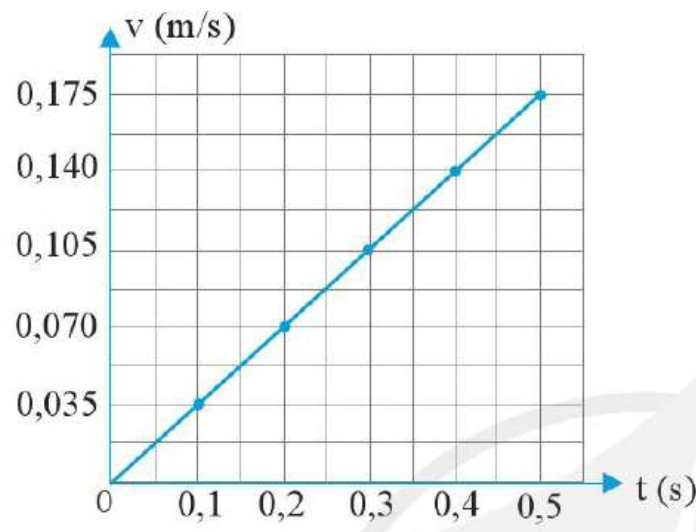
\includegraphics[width=0.3\linewidth]{../figs/VN10-2023-PH-TP008-1}
	\captionof{figure}{Đồ thị vận tốc - thời gian}
	\label{fig:8.1}
\end{center}
Độ dốc của đồ thị $v$ - $t$ cho ta biết độ thay đổi vận tốc của vật theo thời gian, đồ thị càng dốc thì sự thay đổi vận tốc của vật diễn ra càng nhanh.\\
Nếu vật chuyển động thẳng đều thì vận tốc không thay đổi theo thời gian, đồ thị vận tốc - thời gian là một đường thẳng song song với trục hoành $Ot$.
\begin{center}
	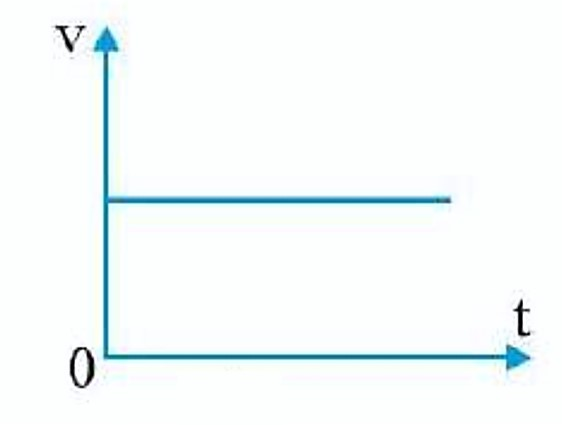
\includegraphics[width=0.2\linewidth]{../figs/VN10-2023-PH-TP008-3}
	\captionof{figure}{Đồ thị vận tốc - thời gian của vật chuyển động thẳng đều.}
\end{center}
\subsubsection{Gia tốc}
Gia tốc là đại lượng đặc trưng cho độ biến thiên của vận tốc theo thời gian. Trong chuyển động thẳng, gia tốc trung bình được xác định theo biểu thức:
$$a_\text{tb}=\dfrac{\Delta v}{\Delta t}=\dfrac{v_2-v_1}{\Delta t}$$
Gia tốc tức thời tại một thời điểm có giá trị bằng độ dốc của tiếp tuyến của đồ thị vận tốc - thời gian $\left(v - t\right)$ tại thời điểm đó.
\begin{center}
	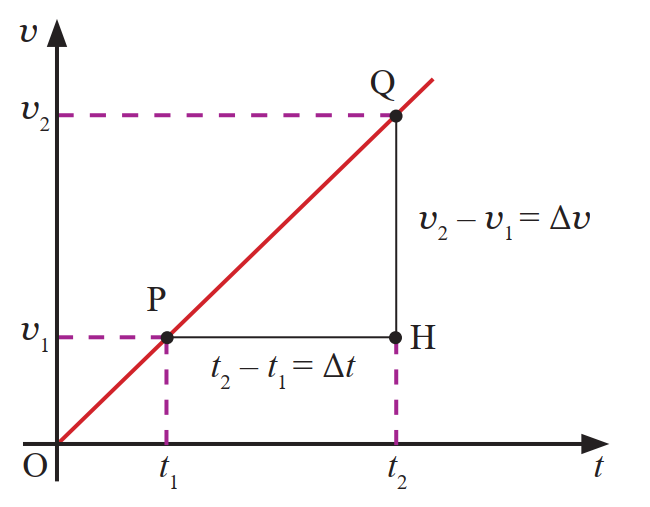
\includegraphics[width=0.3\linewidth]{../figs/VN10-2023-PH-TP008-2}
	\captionof{figure}{Minh hoạ cách xác định gia tốc từ đồ thị vận tốc - thời gian.}
	\label{fig:8.2}
\end{center}
Trong hệ SI, gia tốc có đơn vị là $\si{\meter/\second^2}$.
\subsubsection{Vectơ gia tốc}
Do vận tốc là một đại lượng vectơ nên gia tốc cũng là một đại lượng vectơ. Vectơ gia tốc trung bình được xác định:
$$\overrightarrow{a_\text{tb}}=\dfrac{\Delta \vec{v}}{\Delta t}=\dfrac{\overrightarrow{v_2}-\overrightarrow{v_1}}{\Delta t}$$
Khi $\Delta t$ rất nhỏ, gia tốc trung bình trở thành gia tốc tức thời có:
\begin{itemize}
	\item gốc tại vị trí của vật;
	\item hướng cùng hướng với độ biến thiên vận tốc $\Delta \vec{v}$;
	\item độ dài tỉ lệ với độ lớn của vectơ $\Delta \vec{v}$ theo một tỉ xích xác định.
\end{itemize}
Gia tốc tức thời có thể được đo bằng gia tốc kế.
\subsubsection{Phân biệt một số loại chuyển động thẳng}
\begin{center}
	\begin{tabular}{|m{14em}|m{17em}|m{14em}|}
		\hline
		\thead{$a=0$} & \thead{$a\neq 0$ và bằng hằng số} & \thead{$a\neq 0$ nhưng không phải hằng số}\\
		\hline
		chuyển động thẳng đều, vật có độ lớn vận tốc không đổi. & chuyển động thẳng biến đổi đều, vật có độ lớn vận tốc thay đổi (tăng hoặc giảm) đều theo thời gian. & chuyển động thẳng biến đổi phức tạp.\\
		\hline
	\end{tabular}
\end{center}
\subsection{Vận dụng đồ thị vận $(v - t)$ để xác định độ dịch chuyển}
Độ dịch chuyển của vật trong khoảng thời gian từ $t_1$ đến $t_2$ được xác định bằng phần diện tích giới hạn bởi các đường $v\left(t\right)$, $v=0$, $t=t_1$, $t=t_2$ trong đồ thị $\left(v - t\right)$.\\
\textbf{\textit{Ví dụ:}} Xét vật chuyển động thẳng nhanh dần đều có vận tốc $v_1$ vào thời điểm $t_1=0$ và vận tốc $v_2$ tại thời điểm $t_2$. Độ dịch chuyển của vật trong khoảng thời gian $\Delta t= t_2-t_1$ chính là phần diện tích hình thang $OABD$ trong Hình \ref{fig:8.4}.
\begin{center}
	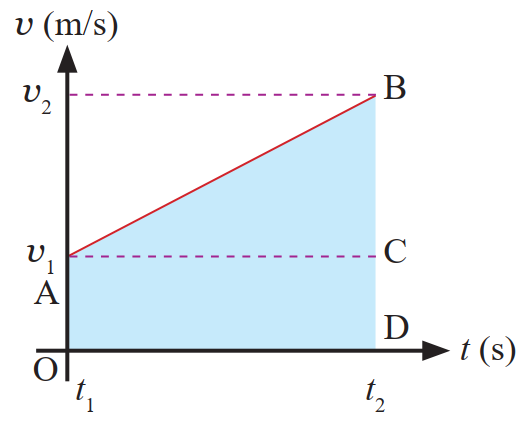
\includegraphics[width=0.3\linewidth]{../figs/VN10-2023-PH-TP008-4}
	\captionof{figure}{Đồ thị $\left(v - t\right)$ của vật chuyển động thẳng biến đổi đều.}
	\label{fig:8.4}
\end{center}
\section{Mục tiêu bài học - Ví dụ minh họa}
\begin{dang}{Phân biệt một số loại chuyển động thẳng }
	\viduii{2}{Trong các chuyển động sau đây, chuyển động nào có giá trị gia tốc không phải là một hằng số trong suốt quá trình chuyển động?
		\begin{enumerate}[label=\alph*)]
			\item Một người đi xe đạp đang tăng tốc đều trên đường thẳng từ trạng thái đứng yên.
			\item Một quả bóng nằm yên trên bàn.
			\item Một thang máy chuyển động từ tầng 2 lên tầng 4 và có dừng đón khách tại tầng 3?
		\end{enumerate}
	Hãy giải thích các câu trả lời mà em đưa ra.
	}
	{	\begin{center}
			\textbf{Hướng dẫn giải}
		\end{center}
	\begin{enumerate}[label=\alph*)]
		\item Người đi xe đạp có gia tốc là một hằng số vì đang chuyển động thẳng nhanh dần đều.
		\item Quả bóng có gia tốc là một hằng số (bằng 0) vì quả bóng không thay đổi trạng thái chuyển động.
		\item Thang máy có gia tốc không phải là một hằng số vì có lúc chuyển động nhanh dần, có lúc chuyển động chậm dần.
	\end{enumerate}
	}
\viduii{2}
{Hình \ref{fig:8.8} là độ thị vận tốc - thời gian trong chuyển động của một bạn đang đi trong siêu thị. Hãy dựa vào đồ thị để mô tả bằng lời chuyển động của bạn đó (khi nào đi đều, đi nhanh lên, đi chậm lại, nghỉ).
\begin{center}
	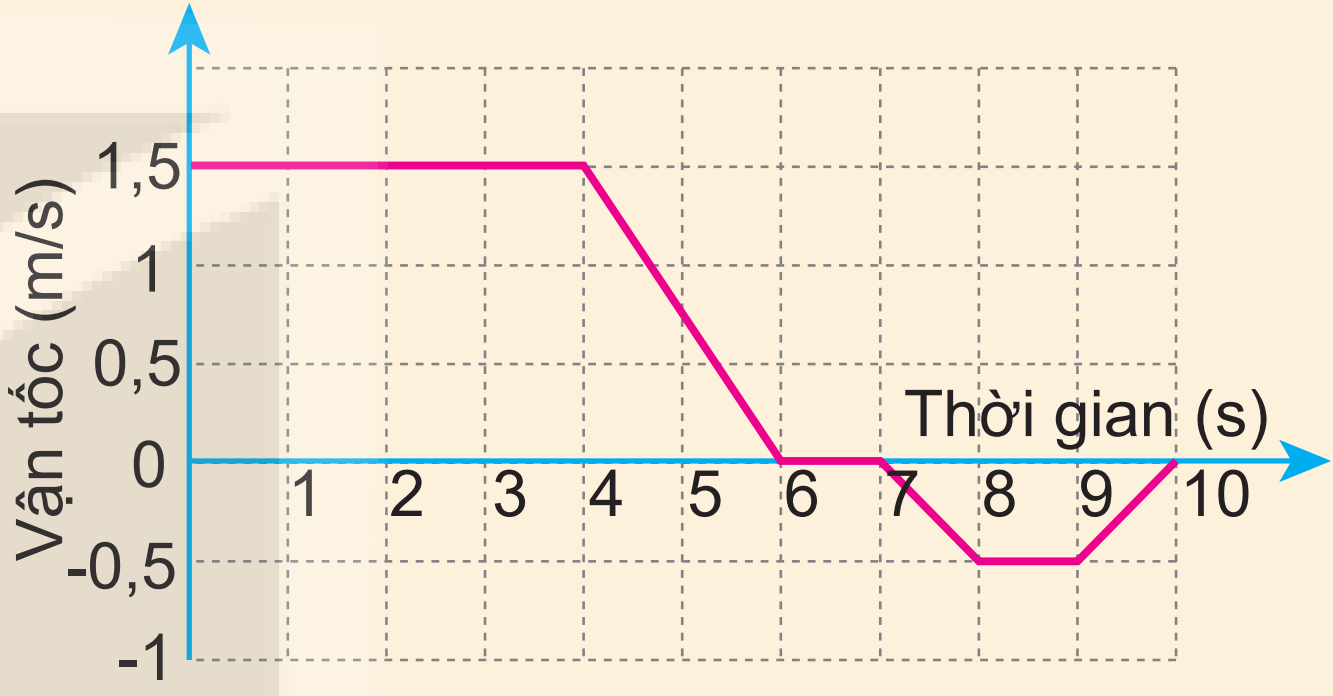
\includegraphics[width=0.4\linewidth]{../figs/VN10-2023-PH-TP008-8}
	\captionof{figure}{Đồ thị $\left(v - t\right)$ của bạn đang đi trong siêu thị.}
	\label{fig:8.8}
\end{center}
}
{\begin{center}
		\textbf{Hướng dẫn giải}
	\end{center}
Mô tả chuyển động của bạn này:
\begin{itemize}
	\item Trong $\SI{5}{\second}$ đầu tiên: bạn đi đều với tốc độ $\SI{1.5}{\meter/\second}$.
	\item Từ thời điểm $\SI{4}{\second}$ đến $\SI{6}{\second}$: bạn đi chậm lại.
	\item Từ thời điểm $\SI{6}{\second}$ đến $\SI{7}{\second}$: bạn đứng yên.
	\item Từ thời điểm $\SI{7}{\second}$ đến thời điểm $\SI{8}{\second}$: bạn đổi chiều chuyển động và đi nhanh dần theo chiều âm.
	\item Từ thời điểm $\SI{8}{\second}$ đến thời điểm $\SI{9}{\second}$: bạn đi đều với tốc độ $\SI{0.5}{\meter/\second}$ theo chiều âm.
	\item Từ thời điểm $\SI{9}{\second}$ đến thời điểm $\SI{10}{\second}$: bạn đi chậm dần theo chiều âm và dừng lại tại thời điểm $\SI{10}{\second}$.
\end{itemize}
}
\end{dang}
\begin{dang}{Vẽ được đồ thị vận tốc – thời gian trong chuyển động thẳng}
	\viduii{2}{Một người lái xe tải đang cho xe chạy trên đường cao tốc với vận tốc không đổi. Khi thấy khoảng cách giữa xe mình với xe chạy phía trước giảm dần, người đó cho xe chạy chậm dần. Tới khi thấy khoảng cách này đột nhiên giảm nhanh, người đó vội đạp phanh để dừng xe. Hãy vẽ đồ thị vận tốc - thời gian mô tả trạng thái chuyển động của xe tải trên.
	}
	{	\begin{center}
			\textbf{Hướng dẫn giải}
		\end{center}
	Chuyển động xe tải qua 3 giai đoạn:
	\begin{itemize}
		\item Giai đoạn từ ban đầu đến thời điểm $t_1$ xe chuyển động với vận tốc không đổi. Đồ thị $\left(v - t\right)$ là một đoạn thẳng song song với trục $Ot$.
		\item Giai đoạn 2 từ thời điểm $t_1$ đến thời điểm $t_2$: xe giảm tốc dần. Đồ thị $\left(v - t\right)$ có hệ số góc âm.
		\item Giai đoạn 3 từ thời điểm $t_2$ đến thời điểm $t_3$: xe giảm tốc nhanh về 0.
	\end{itemize}
	\begin{center}
		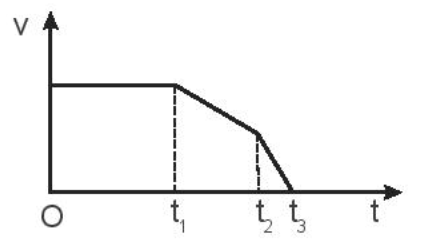
\includegraphics[width=0.3\linewidth]{../figs/VN10-2023-PH-TP008-5}
		\captionof{figure}{Đồ thị vận tốc - thời gian của xe tải.}
	\end{center}
	}
	\viduii{3}{Xét một vận động viên chạy xe đạp trên một đoạn đường thẳng. Vận tốc của vận động viên này tại mỗi thời điểm được ghi lại trong bảng dưới đây.
		\begin{center}
			\begin{tabular}{|c|ccccccccccc|}
				\hline
				$t \left(\si{\second}\right)$ & 0 & 5 & 10 & 15 &20 & 25 & 30 & 35 & 40 & 45 & 50\\
				\hline
				$v \left(\si{\meter/\second}\right)$ & 5 & 5 & 8 & 9 & 10 & 10 & 10 & 12 & 14 & 16 & 16 \\
				\hline
			\end{tabular}
		\end{center}
	Hãy vẽ đồ thị vận tốc – thời gian và mô tả tính chất chuyển động của vận động viên này.
	}
	{	\begin{center}
			\textbf{Hướng dẫn giải}
		\end{center}
		\begin{center}
			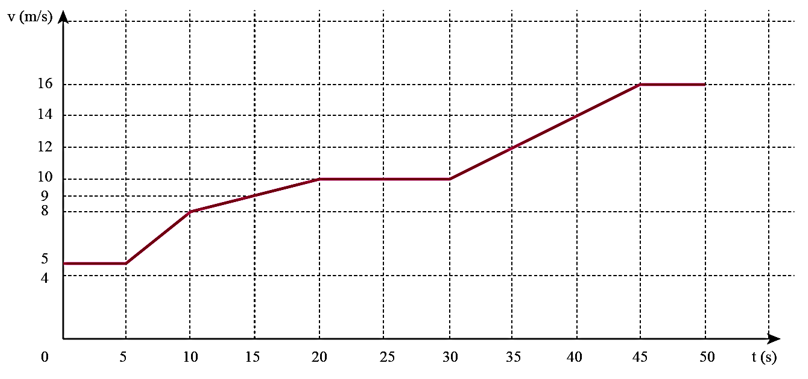
\includegraphics[width=0.8\linewidth]{../figs/VN10-2023-PH-TP008-6}
			\captionof{figure}{Đồ thị vận tốc - thời gian của vận động viên.}
		\end{center}
	Tính chất chuyển động của vận động viên:
	\begin{itemize}
		\item Trong $\SI{5}{\second}$ đầu: chuyển động thẳng đều với vận tốc $\SI{5}{\meter/\second}$.
		\item Trong $\SI{5}{\second}$ tiếp theo: chuyển động thẳng nhanh dần đều với gia tốc $\SI{0.6}{\meter/\second^2}$.
		\item Từ giây thứ 10 đến giây thứ 20: chuyển động thẳng nhanh dần đều với gia tốc $\SI{0.2}{\meter/\second^2}$.
		\item Từ giây thứ 20 đến giây thứ 30: chuyển động thẳng đều với vận tốc $\SI{10}{\meter/\second}$.
		\item Trong $\SI{15}{\second}$ kế tiếp: chuyển động thẳng nhanh dần đều với gia tốc $\SI{0.4}{\meter/\second^2}$.
		\item Sau đó, vận động viên chuyển động thẳng đều với vận tốc $\SI{16}{\meter/\second}$.
		\end{itemize}
	}
	
\end{dang}

\begin{dang}{Vận dụng đồ thị vận tốc – thời gian để tính được độ dịch chuyển và\\gia tốc trong một số trường hợp đơn giản}
	\viduii{3}{Dựa vào đồ thị $\left(v - t\right)$ của vật chuyển động trong Hình \ref{fig:8.7}, hãy xác định gia tốc và độ dịch chuyển của vật trong các giai đoạn:
		\begin{center}
			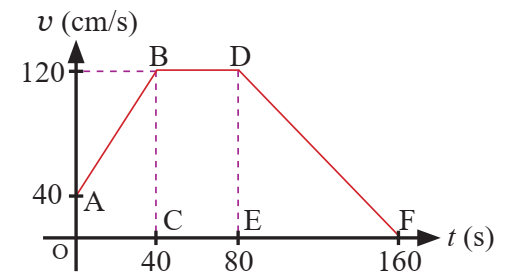
\includegraphics[width=0.5\linewidth]{../figs/VN10-2023-PH-TP008-7}
			\captionof{figure}{Đồ thị $\left(v - t\right)$ của một vật chuyện động.}
			\label{fig:8.7}
		\end{center}
		\begin{enumerate}[label=\alph*)]
			\item Từ $\SI{0}{\second}$ đến $\SI{40}{\second}$.
			\item Từ $\SI{80}{\second}$ đến $\SI{160}{\second}$.
		\end{enumerate}
	}
	{	\begin{center}
			\textbf{Hướng dẫn giải}
		\end{center}
	Chọn chiều dương là chiều chuyển động của vật.\\
	Gia tốc và độ dịch chuyển của vật trong các giai đoạn:
	\begin{enumerate}[label=\alph*)]
		\item $a_1=\dfrac{v_B-v_A}{t_B-t_A}=\dfrac{\left(\SI{120}{\meter/\second}\right)-\left(\SI{40}{\meter/\second}\right)}{\SI{40}{\second}}=\SI{2}{\centi\meter/\second^2}$.\\
		$d_1=\dfrac{1}{2}\cdot\left(OA+BC\right)\cdot OC=\dfrac{1}{2}\cdot\left(\SI{160}{\centi\meter/\second}\right)\cdot \left(\SI{40}{\second}\right)=\SI{3200}{\centi\meter}$.
		\item Tương tự câu a, ta có:
		$a_2 =\dfrac{v_F-v_D}{t_F - t_D}=\dfrac{\left(\SI{0}{\meter/\second}\right)-\left(\SI{120}{\centi\meter/\second}\right)}{\left(\SI{160}{\second}\right)-\left(\SI{80}{\second}\right)}=\SI{-1.5}{\centi\meter/\second^2}$\\
		$d_2=\dfrac{1}{2}\cdot ED \cdot EF=\dfrac{1}{2}\cdot\left(\SI{120}{\centi\meter/\second}\right)\cdot\left(\SI{160}{\second}-\SI{80}{\second}\right)=\SI{4800}{\centi\meter}$.
	\end{enumerate}
	}
\end{dang}

